\newcommand{\obenlinks}{Software Engineering}		% hier Name der Veranstaltung eintragen
% Author: Phil Steinhorst, p.st@wwu.de
% https://github.com/phist91/latex-templates

\documentclass[%
	paper=a4,
	fontsize=10pt,
	ngerman
	]{scrartcl}

% Basics für Codierung und Sprache
% ===========================================================
	\usepackage{scrtime}
	\usepackage{etex}
	\usepackage{shellesc}					% Compiler-Option -shell-escape benutzen!
	\usepackage[final]{graphicx}			% Einbindung von Grafiken
	\usepackage[utf8]{inputenc}				% Dateien sind UTF8-codiert
	\usepackage{babel}						% deutsche Silbentrennung, etc.
	\usepackage[german=quotes]{csquotes}	% deutsche Anführungszeichen mit \enquote{...}
% ===========================================================

% Fonts und Typographie
% ===========================================================
	\usepackage{sourcecodepro}
	\usepackage[default]{sourcesanspro}
	\usepackage{nimbusmononarrow}
	
	\usepackage[babel=true,final,tracking=smallcaps]{microtype}
	\DisableLigatures{encoding = T1, family = tt* } % keine Ligaturen für Monospace-Fonts
	\usepackage{ellipsis}
% ===========================================================

% Farben
% ===========================================================
	\usepackage[usenames,x11names,final]{xcolor}
% ===========================================================

% Mathe-Pakete und -Einstellungen
% ===========================================================
	\usepackage{mathtools}					% Tools zum Setzen von Formeln
	\usepackage{amssymb}					% übliche Mathe-Symbole
	\usepackage[bigdelims]{newtxmath}		% moderne Mathe-Font
	\allowdisplaybreaks						% seitenübergreifende Rechnungen
	\usepackage{bm}							% math bold font
	\usepackage{wasysym}					% noch mehr Symbole
	\usepackage{forest}
	\usepackage{pifont}% http://ctan.org/pkg/pifont
% ===========================================================

% TikZ
% ===========================================================
	\usepackage{tikz}
	\usepackage{tikz-cd}					% kommutative Diagramme
	\usetikzlibrary{arrows.meta}			% mehr Pfeile!
	\usetikzlibrary{calc}					% TikZ kann rechnen
	\tikzset{>=Latex}						% Standard-Pfeilspitze
% ===========================================================

% Seitenlayout, Kopf-/Fußzeile
% ===========================================================
	\usepackage{scrpage2}
	\pagestyle{scrheadings}
	\usepackage[top=3cm, bottom=3cm, left=2.5cm, right=2cm]{geometry}
	\clearscrheadfoot 
	\setheadsepline{0.4pt}			 					% Linie in Kopfzeile
	\setfootsepline{0.4pt}								% Linie in Fußzeile
	\setkomafont{pagehead}{\bfseries}					% Schriftart Kopfzeile
	\setkomafont{pagefoot}{\normalfont\footnotesize}	% Schriftart Fußzeile 
	\cfoot{\thepage}									% Seitenzahl unten Mitte
	\lohead{\obenlinks}	% Titel oben links
	\raggedbottom							% Flattersatz
	\usepackage{setspace}					% erweiterte Abstandsoptionen
	\onehalfspacing							% Zeilenabstand 1.5-fach
	\setlength{\parindent}{0pt}				% Einrückung neuer Absätze
	\setlength{\parskip}{0.5\baselineskip}	% Abstand neuer Absätze
% ===========================================================

% Hyperref für Referenzen und Hyperlinks
% ===========================================================
	\usepackage[%
		hidelinks,
		pdfpagelabels,
		bookmarksopen=true,
		bookmarksnumbered=true,
		linkcolor=black,
		urlcolor=SkyBlue2,
		plainpages=false,
		pagebackref,
		citecolor=black,
		hypertexnames=true,
		pdfborderstyle={/S/U},
		linkbordercolor=SkyBlue2,
		colorlinks=false,
		backref=false]{hyperref}
	\hypersetup{final}
% ===========================================================

% Listen und Tabellen
% ===========================================================
	\usepackage{multicol}
	\usepackage[shortlabels]{enumitem}
	\setlist{itemsep=0pt}
	\setlist[enumerate]{font=\sffamily\bfseries}
	\setlist[itemize]{label=$\triangleright$}
	\usepackage{tabularx}
% ===========================================================

% listings
% ===========================================================
\usepackage{listingsutf8}
\lstset{
	belowcaptionskip=1\baselineskip,
	breaklines=true,
	showstringspaces=false,
	basicstyle=\ttfamily,
	keywordstyle=\bfseries\color{green!40!black},
	commentstyle=\itshape\color{purple!40!black},
	stringstyle=\color{orange},
	numbers=left,
	numberstyle=\footnotesize\ttfamily\color{gray},
	inputencoding=utf8/latin1,
	tabsize=4,
}

%%%%%%%%%%%%%%%%%%%%%%%%%%%%%%%%%%%%%%%%%%%%%%%%%%%%%%%%%%%
%%% Ab hier folgen nur noch vordefinierte Shortcuts %%%
%%%%%%%%%%%%%%%%%%%%%%%%%%%%%%%%%%%%%%%%%%%%%%%%%%%%%%%%%%%

\newcommand{\BB}{\mathbb{B}}
\newcommand{\CC}{\mathbb{C}}
\newcommand{\NN}{\mathbb{N}}
\newcommand{\QQ}{\mathbb{Q}}
\newcommand{\RR}{\mathbb{R}}
\newcommand{\ZZ}{\mathbb{Z}}
\newcommand{\oh}{\mathcal{O}}

\newcommand{\ol}[1]{\overline{#1}}
\newcommand{\wt}[1]{\widetilde{#1}}
\newcommand{\wh}[1]{\widehat{#1}}

\DeclareMathOperator{\id}{id} 				% Identität
\DeclareMathOperator{\pot}{\mathcal{P}}		% Potenzmenge

% Klammerungen und ähnliches
\DeclarePairedDelimiter{\absolut}{\lvert}{\rvert}		% Betrag
\DeclarePairedDelimiter{\ceiling}{\lceil}{\rceil}		% aufrunden
\DeclarePairedDelimiter{\Floor}{\lfloor}{\rfloor}		% aufrunden
\DeclarePairedDelimiter{\Norm}{\lVert}{\rVert}			% Norm
\DeclarePairedDelimiter{\sprod}{\langle}{\rangle}		% spitze Klammern
\DeclarePairedDelimiter{\enbrace}{(}{)}					% runde Klammern
\DeclarePairedDelimiter{\benbrace}{\lbrack}{\rbrack}	% eckige Klammern
\DeclarePairedDelimiter{\penbrace}{\{}{\}}				% geschweifte Klammern
\newcommand{\Underbrace}[2]{{\underbrace{#1}_{#2}}} 	% bessere Unterklammerungen
% Kurzschreibweisen für Faule und Code-Vervollständigung
\newcommand{\abs}[1]{\absolut*{#1}}
\newcommand{\ceil}[1]{\ceiling*{#1}}
\newcommand{\flo}[1]{\Floor*{#1}}
\newcommand{\no}[1]{\Norm*{#1}}
\newcommand{\sk}[1]{\sprod*{#1}}
\newcommand{\enb}[1]{\enbrace*{#1}}
\newcommand{\penb}[1]{\penbrace*{#1}}
\newcommand{\benb}[1]{\benbrace*{#1}}
\newcommand{\stack}[2]{\makebox[1cm][c]{$\stackrel{#1}{#2}$}}
\usepackage{listings}

\begin{document}
	\begin{center}
		\begin{tabular}{|rlp{4cm}rll|}
		\hline
		 \textbf{Übungsblatt:} & 5 &   & \textbf{1. Abgabepartner:} & Matthias Wolff & (458 766)  \\
		        & & & \textbf{2. Abgabepartner:} & Anton Mende & (461 328) \\
		        & & & \textbf{2. Abgabepartner:} & Anika Herbermann & (461 655) \\ \hline
		\end{tabular}
	\end{center}
\section*{Aufgabe 15}	
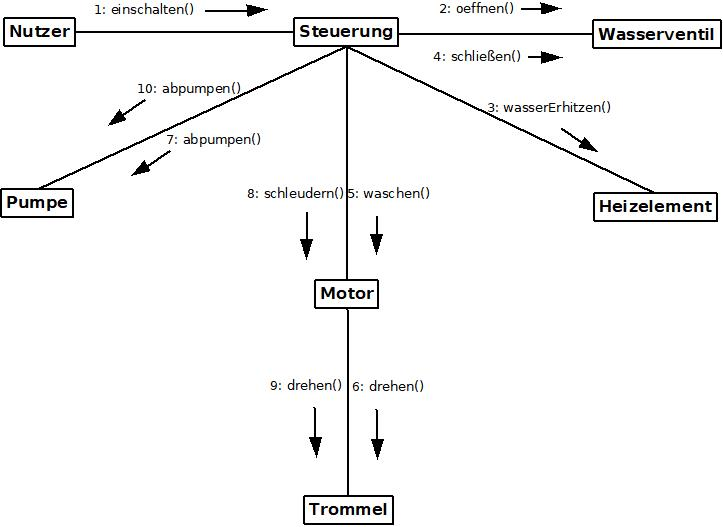
\includegraphics[scale=0.7]{Aufgabe_15.jpeg}
\newpage
\section*{Aufgabe 16}
\subsection*{a)}
\begin{itemize}
\item[-] \textbf{parallele Verarbeitung}: Die Fön-Software muss sowohl Lüfterdrehzahl als auch Heizelementtemperatur gleichzeitig steuern\\
\item[-] \textbf{Einbenutzerfähigkeit}: Ein Fön wird immer nur von einer einzigen Person gleichzeitig benutzt\\
\item[-] \textbf{Schichten}: Der Fön muss sich nicht zu einem Server verbinden. Somit muss nur die Client-Schicht entwickelt werden, die die komplette Steuerung des Föns übernimmt\\
\item[-] \textbf{Notwendigkeit verschiedener Plattformen}: Das System soll nur als Embedded-System fest im Fön verbaut laufen. Somit muss nur für diese eine Plattform entwickelt werden
\item[-] \textbf{Wiederverwendung vorhandener Bausteine}: Die Fön-Software benötigt keine Wiederverwendung vorhandener Bausteine, da lediglich Temperatur und Lüfterdrehzahl geregelt werden müssen. Dafür kann man keine Bausteine wiederverwenden.\\
\item[-] \textbf{Hilfesystem}: Die Fön-Bedienung ist intuitiv genug, sodass kein Hilfesystem benötigt wird.
\item[-] \textbf{DBMS}: Der Fön muss keine Daten persistent speichern. Somit entfällt die Benutzung eines DBMS\\
\item[-] \textbf{Benutzerschnittstelle}: Die Benutzerschnittstelle wird durch Hardware-Schalter realisiert, durch die der Benutzer Eingaben zur gewünschten Lufttemperatur und Lüfterdrehzahl tätigen kann.\\
\item[-] \textbf{Rückgriffe auf sonstige Dienstleistungen}: entfallen, da die Fön-Software nicht sehr komplex ist, sodass Rückgriffe auf sonstige Dienstleistungen nicht nötig sind.\\
\end{itemize}
\newpage
\subsection*{b)}
\begin{itemize}
\item[-] \textbf{sequentielle Verarbeitung}: Der Kunde soll seine Pizza Schritt für Schritt nacheinander konfigurieren und die Konfiguration soll danach an den Unternehmens-Server geschickt werden. Es läuft alles einzeln nacheinander ab, somit wird keine Parallelität / Nebenläufigkeit benötigt.\\
\item[-] \textbf{Einbenutzerfähigkeit}: Die Software auf dem Smartphone wird jeweils nur von einem einzigen Kunden benutzt. Das Softwaresystem auf dem Unternehmens-Server muss mehrbenutzerfähig sein, die Handy-App jedoch nicht.\\
\item[-] \textbf{Schichten}: Die Software läuft lokal auf einem Smartphone als Client. Erst beim Abschluss der Konfiguration sendet der Client die fertig konfigurierte Pizza an einen Unternehmens-Server. Die zu entwickelnde Software ist also Client-Software.
\item[-] \textbf{Notwendigkeit verschiedener Plattformen}: Die Software muss auf allen gängigen Smartphones laufen (Android, Apple, WindowsPhone,...)
\item[-] \textbf{Wiederverwendung vorhandener Bausteine}:   Die Auswahl-Menüs für Zutaten, Pizzaboden, Pizzasoße, etc. können mit anderen Werten wiederverwendet werden, da der strukturelle Aufbau der graphischen Auswahl-Menüs jeweils gleich ist.
\item[-] \textbf{Hilfesystem}: Ein Hilfesystem ist nicht zwingend erforderlich, da die App den Kunden intuitiv durch die Konfiguration seiner Pizza führt und Schritt für Schritt nach Angaben fragt.\\
\item[-] \textbf{DBMS}: Die Software, die auf dem Smartphone läuft sollte zur besseren Bedienbarkeit die persönlichen Daten des Kunden wie Name, Adresse, Telefonnummer, etc. lokal speichern, sodass der Kunde diese nicht jedes Mal von Hand eingeben muss. Da dies nur ein einziger Eintrag ist, ist hierfür ein DBMS nicht nötig. Zusätzlich müssen die möglichen Wahloptionen für Zutaten, Pizzaböden und Soßen in einer relationalen Datenbank gespeichert werden.\\
\item[-] \textbf{Benutzerschnittstelle}: Die Benutzerschnittstelle soll in Form einer GUI realisiert werden
\item[-] \textbf{Rückgriff auf sonstige Dienstleistungen}: GUI-Framework zur Erstellung der Benutzerschnittstelle, Netzwerk-Bibliothek zum Senden der Pizza-Konfiguration über 5G an den Unternehmens-Server. Für das Hilfesystem könnte ebenfalls ein Halbfabrikat verwendet werden.
\end{itemize}
\newpage
\subsection*{c)}
\begin{itemize}
\item[-] \textbf{sequentielle Verarbeitung}: Jeder Registrierungs bzw. Bezahlvorgang wird nacheinander abgearbeitet.
\item[-] \textbf{Mehrbenutzerfähigkeit}: Mehrere Kunden werden das System gleichzeitig nutzen
\item[-] \textbf{Schichten}: Die Registrierung erfolgt in einer Web-Applikation. Als Client dient hierbei ein Smartphone bzw. Rechner des jeweiligen Kunden, der sich registrieren möchte. Die Bezahlung erfolgt am Automaten als Client, der den Bezahlvorgang mit dem Bezahlsystem als Server abwickelt.
\item[-] \textbf{Notwendigkeit verschiedener Plattformen}: Die Software zur Registrierung läuft in einem Browser (PHP, HTML). Die Software zum Bezahlen läuft lokal auf dem Pizzaautomaten.
\item[-] \textbf{Wiederverwendung vorhandener Bausteine}: entfällt, da keine Teile des Systems sich dafür ähnlich genug sind.
\item[-] \textbf{Hilfesystem}: Ein Hilfesystem für den Kunden ist wünschenswert, um Fragen bei der Registrierung, beim Bezahlvorgang oder beim Verlust der Karte zu beantworten.\\
\item[-] \textbf{DBMS}: Die personenbezogenen Daten sollen vertraulich in einem relationalen DBMS gespeichert werden. Zusätzlich sollten getätigte Bestellungen gespeichert werden. 
\item[-] \textbf{Benutzerschnittstelle}: Die Benutzerschnittstelle wird als GUI realisiert, die den Kunden im Browser durch den Registrierungsvorgang leitet. Am Automaten wird auf dem vorhandenen Bildschirm der Status der kontaktlosen Bezahlung angezeigt.
\item[-] \textbf{Rückgriff auf sonstige Dienstleistungen}: Es kann auf ein Halbfabrikat zur datenschutzkonformen Speicherung der personenbezogenen Daten zurückgegriffen werden, das die Daten (eventuell verschlüsselt) in einer Datenbank ablegt. Zusätzlich kann eine Bibliothek zum kontaktlosen Auslesen der Karten verwendet werden. Für das Hilfesystem kann ebenfalls ein Halbfabrikat verwendet werden.
\end{itemize}
\newpage
\section*{Aufgabe 17}
\lstset{basicstyle=\tiny ,language=Java}
\subsection*{a)}
\lstinputlisting{Aufgabe17a.java}
\newpage
\subsection*{b)}
\lstinputlisting{Aufgabe17b.java}
\end{document}
